\chapter{Grundlagen}

In diesem Kapitel werden alle verwendeten Komponenten und Technologien kurz erläutert.

\section{LR-WPAN - IEEE 802.15.4}

LR-WPAN steht für \grqq Low Rate - Wireless personal area network \grqq{}. Es handelt sich um ein drahtloses geschlossenes Netzwerk, welches für 
niedrige Datenraten ausgelegt ist. Der Standard definiert den Physical Layer sowie den Media-Access Layer und ist damit die Grundlage von ZigBee, Thread und 6LowPAN.
Im Standard sind mehrere Modulationsverfahren sowie Frequenzbereiche definiert. Peer-to-Peer ist Teil des Standards. Im vergleich zum 802.1d Standard fallen 
vorallem die kürzeren Adressen auf. Dadurch kann die für den Anwendungsbereich wertvolle Bandbreite und Rechenleistung reduziert werden. 

\section{ZigBee}

Die ZigBee Alliance wurde durch ein Konsortium von Herstellern gegründet, um einen einheitlichen Übertragungstandard
im Bereich Heimautomatisierung voranzubringen. ZigBee basiert auf dem offenem 802.15.4 Standard, bringt allerdings zusätzliche Komponenten mit die nicht in einem IEEE
Standard definiert sind.
ZigBee ist in Form von weiteren Protokollschichten implementiert, welche auf IEEE 802.15.4 aufsetzen. ZigBee nutzt DSSS, also Frequenzspreizung als Modulationsverfahren.
Die genutzten Kanäle, 11 bis 26, liegen im 2,4 Ghz Band. Zigbee interferiert damit mit WLAN.

\begin{figure}[H]
  \centering
  \includegraphics[width=1\textwidth]{media/Zigbee Stack.jpg}
  \caption{ZigBee Protocoll Stack \\ Bildquelle: \url{https://www.researchgate.net/figure/IEEE820154-ZigBee-protocol-stack-architecture_fig2_265150617}}
\end{figure}

Der Anwendungsbereich für ZigBee ist die Heimautomatisierung. Geräte können zentral gesteuert und überwacht werden. 
Markante Eigenschaft von ZigBee ist, dass die Geräte keine direkte Funkverbindung
zu einem zentralen Controller brauchen. Andere Geräte können als Router fungieren, und damit die Reichweite erhöhen. Sende- und Empfangsleistung
ist vorallem bei kleinen Batteriebetriebenen Geräten oft der einschränkende Faktor.


\section{Texas Instruments CC Chips}

Texas Instruments bietet ein Spektrum von Microcontrollern, die sich mit entsprechender Firmware für ZigBee Geräte 
nutzen lassen. Kleinere Varianten können in Endgeräten wie Lampen und Thermostate, größere als Koordinator selbst verwendet werden.

Die aktuelle Chipfamilie TexasInstruments CC26XX:

\begin{figure}[H]
  \centering
  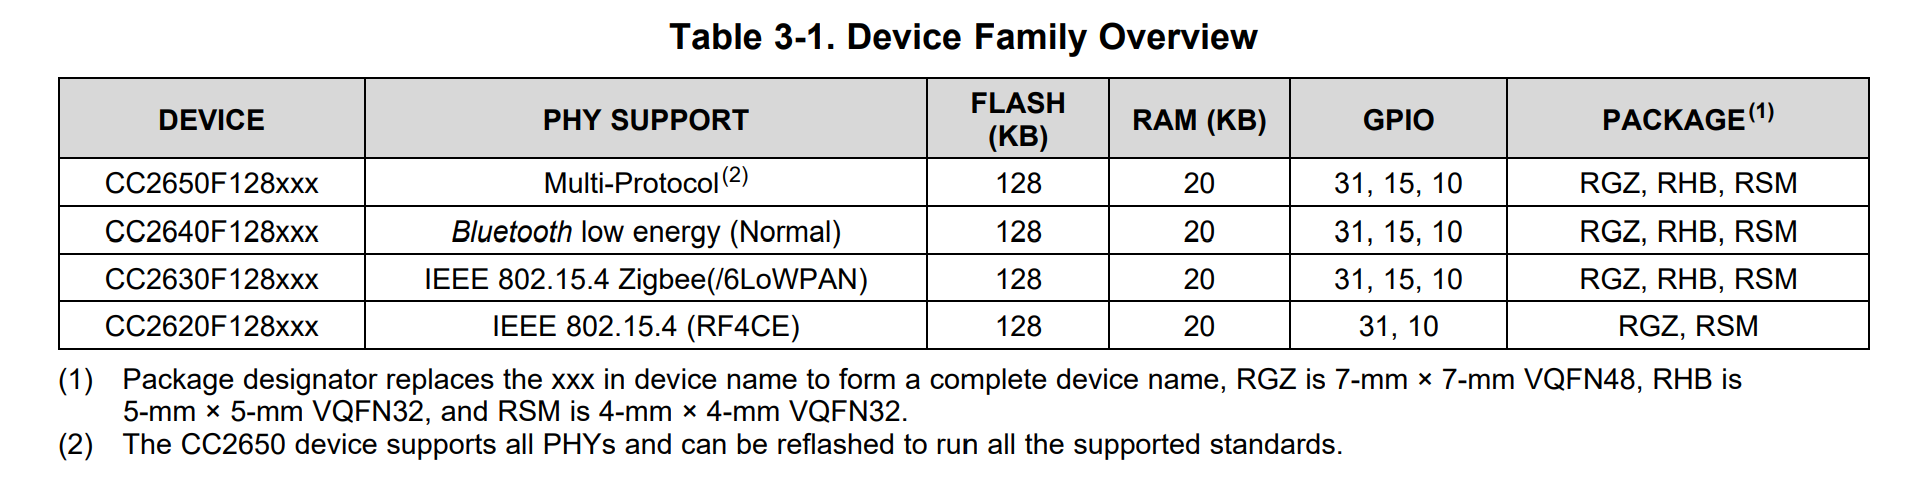
\includegraphics[width=1\textwidth]{media/table26xx.png}
  \caption{TI Device Family}
\end{figure}

Als Koordinator werden die Leistungsfähigeren Chips aus der 265X Reihe eingesetzt. ZigBee Geräte nutzen in einigen
Anwendungen Bluetooth LE zur Koppelung, daher ist die Unterstüzung diesen Protokolls sinnvoll.

\begin{figure}[H]
  \centering
  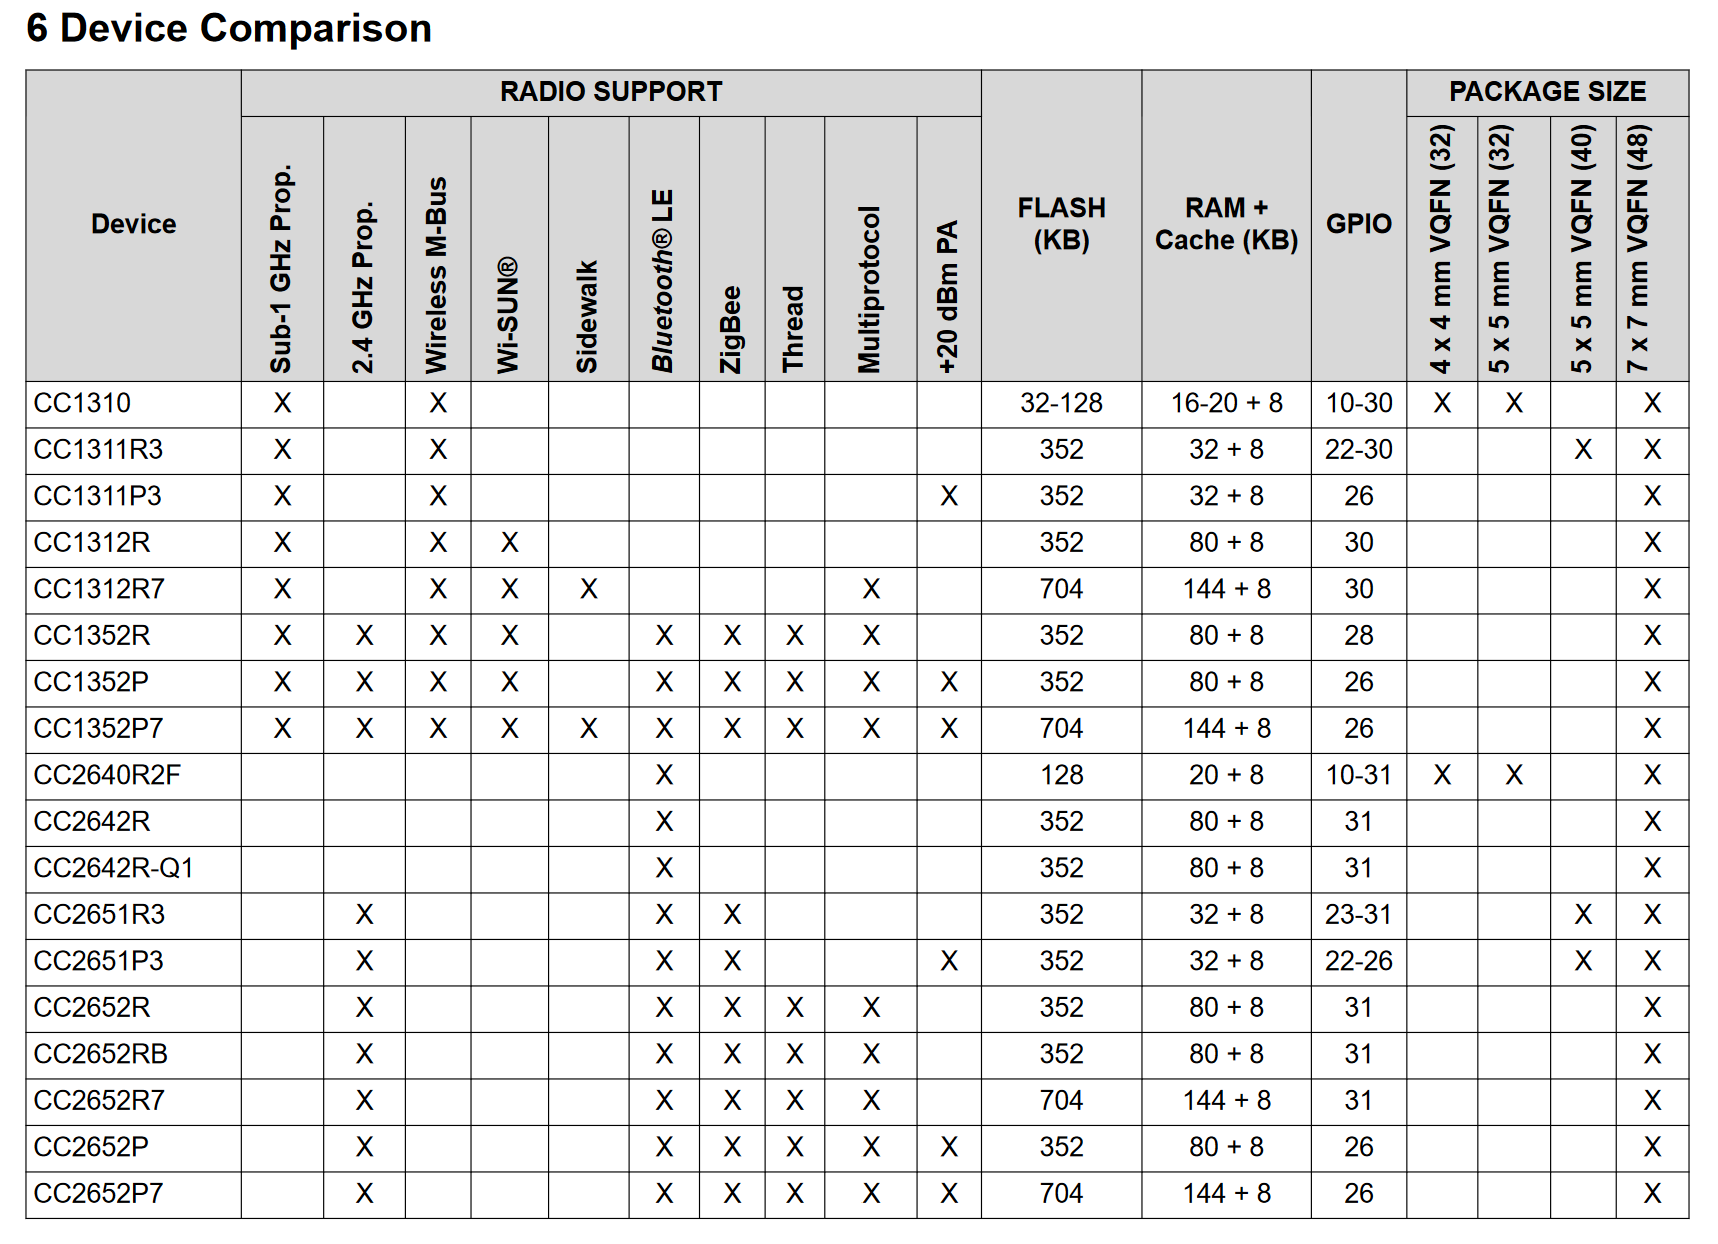
\includegraphics[width=1\textwidth]{media/table265x.png}
  \caption{TI CC 265X Serie}
\end{figure}

In der Tabelle sind die unterstützten Protokolle der einzelnen Modelle sowie deren Leistungsfähigkeit aufgeführt.
Es ist anzumerken, dass die größeren Modelle schon den Standard Thread unterstützen, der vermutlich durch das
Projekt \grqq Matter\grqq{} erheblich an Bedeutung gewinnen wird.

Texas Instruments stellt als Basis für ZigBee Anwendungen eine Z-Stack Bibliothek zur Verfügung. Diese stellt alle grundlegenden 
Funktionen um das ZigBee Protokoll zu implementieren. Mit Texas Instruments Code Composer Studio steht eine IDE bereit,
um den Entwicklungsprozess zu unterstützen. Auf den entsprechend Leistungsfähigeren Chips lassen sich in freie Speicherbereiche noch zusätzliche
Funktionalitäten einprogrammieren. Die Chips können mit Programmierboards des Herstellern programmiert werden. Alternativ kann man
günstig einen USB-Stick mit aufgelöteten CC Chip erwerben, und auch diesem mit entsprechenden Tools programmieren.

Weiter Informationen: \url{https://www.ti.com/tool/Z-STACK#overview}

In dem OpenSource Projekt \grqq zigbee2mqtt \grqq{} werden ausschließlich Chips von Texas Instruments unterstützt. Die meißten gängigen Anbieter von Microchips 
haben entsprechende Modelle im Angebot. 

\section{Versuchshardware}

\subsection{RaspberryPi}

Der RaspberryPi ist ein ARM basierter Computer im Mini-Format. Er dient in diesem Versuch als Applikationsserver und gleichzeitig als Versuchs-PC, 
auf dem der Versuch durchgeführt wird. Die eingesetzten Anwendungen sind 
als Webservice implementiert und werden per Docker Containerisierung ausgerollt.

Der RaspberryPi besitzt die PC typtischen Schnittstellen wie Ethernet, HDMI, sowie USB. Als Festspeicher wird eine
SD-Karte eingestzt. 

Auf dem RaspberryPi wird das Linux-basierte Betriebssystem RaspbianOS. Dies ist eine von den Entwicklern des RaspberryPis eigenentwickelte und für den RaspberryPis
angepasste Linux-Distribution. Es baut auf Ubuntu auf.

\subsection{RaspberryPi Zigbee Hat}

Als Zigbee Koordinator wird ein auf dem TI CC2652 basierendem RaspberryPi Hat vom Hersteller \grqq cod.m \grqq{} eingesetzt. Dieser wurde vom Hersteller
für den Einsatz mit \grqq homegear \grqq{} oder \grqq zigbee2Mqtt \grqq{} entwickelt. Ein Datenblatt und Bedienungsanleitung sind im Anhang.

\subsection{CC2531 Sniffer Stick}

Mit diesem Stick wird die ZigBee Kommunikation in des Versuchsnetzwerkes mitgeschnitten.
Der Stick basiert auf einem leistungsschwachen Chip, der mit entsprechender Firmware Pakete mitschneiden kann. 

Als Treiber wird ein in C geschriebenes Programm verwendet, welches es ermöglicht den Stick direkt als Interface in Wireshark hinzuzufügen. Der Quellcode findet sich in 
GitHub unter https://github.com/andrebdo/wireshark-cc2531. Hier ist auch eine Anleitung zum kompilieren. Die hieraus entstehende ausführbare Datei muss in entsprechenden
Wireshark Ordner kopiert werden, und kann anschließend als Interface ausgewählt werden. Die Funktion nennt sich bei Wireshark \grqq extcap \grqq{}.

todo: Screenshot wireshark

\subsection{Phillips Hue Komponenten}

Unter dem Namen \grqq Hue \grqq{} vertreibt Phillips eine Reihe intelligenten Endgeräten sowie entsprechenden Komponenten um diese zu steuern.
Die Phillips Hue Serie setzt auf ZigBee sowie Bluetooth LE. Unter anderem sind Lampen, Steckdosen, eine Bridge sowie eine App verfügbar.
Die Bridge stellt bei traditionellen Lösungen die Schnittstelle zwischen der ZigBee Kommunikation zwischen den Geräten und der IP Kommunikation zu beispielßweiser einer Smartphone
App.  Die Geräte sind Kompatibel zu dem Software-Gateway zigbee2mqtt, benutzen also keine speziellen Schlüssel oder ähnliches.
Die Lampen werden in dem Versuch als Demonstrationsobjekte eingesetzt. Sie können Ein- und Ausgeschaltet werden, sowie gedimmt werden. Zusätzlich wird eine
Phillips Hue Fernbedienung verwendet, die zur Steuerung der Lampen genutzt wird.

\section{Eingesetzte Software}

\subsection{Raspbian OS}

RaspbianOS ist eine leichtgewichtige Linux Distribution, welche direkt vom Hersteller des RaspberryPis speziell auf die Bedürfnisse des Board angepasst ist. Es enthällt eine
Desktop Umgebung sowie grundlegende Pakete. Es basiert auf Debian, damit sind entsprechenden reichhaltige Paketquellen verfügbar. 

\subsection{Docker}

Docker ist eine Containerisierungslösung, um Anwendungen containerisiert auf Linux-Servern ausführen zu können. Docker reduziert erheblich den Aufwand 
Anwendungen zu betreiben. Da alle notwendigen Abhängigkeiten mit einem Container mitgeliefert werden, ist eine Installation meißt komplikationsfrei.
Prozesse laufen in eigenen Namespaces und sind dadurch abgekoppelt von anderen Containern sowie dem Hostbetriebssystem. Im Unterschied zur Virtualisierung werden
einige Ressourcen gemeinsam genutzt. Dadurch ist die Effizienz höher als bei taditioneller Virtualisierung, bei der meißt ein vollständiges Betriebssystem virtualisiert wird.

\subsection{Docker-Compose}

Docker-Compose ist ein Tool, um große Containerumgebungen im Textformart, hier \grqq YAML \grqq{} zu definieren.
Ein Container kann entweder per Docker-CLI mit entsprechenden Parametern gestartet werden:
\begin{lstlisting}
  docker run hello-world -v ./home:/home -p 80:80
\end{lstlisting}

Durch diesen Befehl wird der Container \grqq hello-world \grqq aus dem Docker Repository geladen und anschließend gestartet. In diesem ist ein einfacher Webserver der bei
Aufruf ein \grqq Hello world ! \grqq{} zurückgibt implementiert. Zusätzlich wird der Ordner \grqq home \grqq{} in den Container gemountet. Dieser bleibt auch bei einem
erneuten Laden des Containers persistent. Dies wird beispielweiße für Konfigurationsdateien oder andere persistente Dateien genutzt. Um den Container auch auf der Schnittstelle
des Host-Systems verfügbar zu machen, wird der Port 80 auf den Container Port 80 gemappt. Die Funktionsweiße wird später erläutert.

Alternativ zu der Docker-CLI lässt sich der Zielzustand auch beschreiben:

\begin{lstlisting}
version: '3'
services:
  helloworld:
    container_name: helloworld
    image: hello-world
    ports:
      - 80:80
    volumes:
      - ./home:/home
    restart: unless-stopped
\end{lstlisting}

Mit einem 
\begin{lstlisting}
  docker-compose up -d
\end{lstlisting}

errhält man das selbe Ergebniss wie mit dem vorher gezeigtem CLI Befehl.

\subsection{zigbee2mqtt}

zigbee2mqtt ist ein offenes Softwareprojekt und am besten mit \grqq Software-Zigbee-Gateway\grqq{} beschrieben werden. Es übernimmt die Funktionalität, die normalerweise entsprechende
 Bridges der Hersteller übernehmen. Während traditionelle Bridges, wie zum Beispiel die Phillips Hue Bridge eine REST API zur Verfügung stellen um mit ihren
Apps zu kommunizieren, macht zigbee2mqtt die Geräte per mqtt nach außen verfügbar. Auf abstrakter Ebene bedeutet dies, das es ein Gateway zwischen einem Zigbee Netzwerk und
einem traditionellen IPv4 Netzwerk ist. Zur Steuerung und Visualisierung lassen sich per MQTT Anwendungen wie \grqq Homeassistant\grqq{} oder \grqq OpenHUB\grqq{} oder auch entsprechende
Eigenentwicklungen einsetzen. \grqq zigbee2mqtt\grqq{} greift direkt auf den \grqq cod.m\grqq{} ZigBee Adapter zu.

Quellcode und Dokumentation: \url{https://github.com/Koenkk/zigbee2mqtt}
Homepage: \url{https://www.zigbee2mqtt.io/}

\grqq zigbee2mqtt\grqq{} verwaltet ein Zigbee Netzwerk und ermöglicht es Drittanwendungen, die Geräte in diesem ZigBee Netz zu Steuern. Wird ein neues Device ins das Netzwerk eingefügt,
kündigt zigbee2mqtt das Gerät per MQTT an, und gibt nach erfolgreichem Interview alle Cluster an.

todo: Screenshot MQTT

Zigbee2Mqtt verwaltet drei Datenbanken, welche die Funktionsweiße deutlich machen. Viele Funktionen, wie zum Beispiel die Verwaltung von Routingtabellen und
Verschlüsselung der Kommunikation sind direkt in der Hardware implementiert. Diese Funktionen lassen sich wie in der im Punkt TI CC Firmware gezeigen API Steuern und Abfragen.
Zigbee2mqtt verwaltet in einer eigenen Datenbank die Geräte im Netzwerk sowie deren Eigenschaften.
Folgende Datensätze finden sich in der Anwendung:

\textbf{coordinator-backup.json}\\

Wie der Name sagt, sind hier die für die Initialisierung beim Start des Koordinators wichtigen Informationen abgelegt. Dies beinhaltet alle dem Netzwerk zugehörigen Geräte.
Durch löschen dieser Datei wird das Netzwerk vollständig zurückgesetzt. Die einzelnen Teilnehmer müssen dann manuell per Touchlink oder nach herstellerspezifischem Verfahrem
zurückgesetzt werden, um wieder einem neuen Netzwerk beitreten zu können.


\begin{lstlisting}
  {
    "metadata": {
      "format": "zigpy/open-coordinator-backup",
      "version": 1,
      "source": "zigbee-herdsman@0.14.103",
      "internal": {
        "date": "2023-05-04T19:48:28.936Z",
        "znpVersion": 1
      }
    },
    "stack_specific": {
      "zstack": {
        "tclk_seed": "69a6670050d8354347405537724e1a81"
      }
    },
    "coordinator_ieee": "00124b0026b748c8",
    "pan_id": "1a62",
    "extended_pan_id": "00124b0026b748c8",
    "nwk_update_id": 0,
    "security_level": 5,
    "channel": 11,
    "channel_mask": [
      11
    ],
    "network_key": {
      "key": "01030507090b0d0f00020406080a0c0d",
      "sequence_number": 0,
      "frame_counter": 5552161
    },
    "devices": [
      {
        "nwk_address": "9a3b",
        "ieee_address": "0017880104b9359d",
        "is_child": false,
        "link_key": {
          "key": "87b4d0a2668847d8a876fe4454bf654e",
          "rx_counter": 0,
          "tx_counter": 121
        }
      },
  ...  
  \end{lstlisting}

  Hier liegen die wichtigsten Parameter über das ZigBee Netzwerk sowie Eckdaten über alle Teilnehmer ab.

  \textbf{state.json}\\

  In dieser Datei sind alle aktuellen Zustände Geräte im Netzwerk hinterlegt. Sie dient dazu, bei einem Neustart des Koordinators den letzten Zustand wieder herzustellen.

  \begin{lstlisting}
    ...
    "0xbc33acfffe9587ed": {
        "brightness": 15,
        "state": "OFF",
        "color_mode": "color_temp",
        "color_temp": 360,
        "linkquality": 40,
        "color": {
            "x": 0.4542,
            "y": 0.4092
        },
        "do_not_disturb": false
    ...
  \end{lstlisting}
  \textbf{database.db}\\

  Dies ist die zentrale Datenbank von zigbee2mqtt. Da SQLite eingesetzt wird, lässt sich auch hier der Inhalt wie bei einer Textdatei einfach auslesen.
  Es liegt für jedes Device ein Datensatz ab.

  Datensatz des Koordinators:
  \begin{lstlisting}
{"id":1,"type":"Coordinator","ieeeAddr":"0x00124b0026b748c8","nwkAddr":0,"manufId":0,"epList":[1,2,3,4,5,6,8,10,11,12,13,47,110,242],
"endpoints":{"1":{"profId":260,"epId":1,"devId":5,"inClusterList":[],"outClusterList":[],"clusters":{},"binds":[],"configuredReportings":[],
"meta":{}},"2":{"profId":257,"epId":2,"devId":5,"inClusterList":[],"outClusterList":[],"clusters":{},"binds":[],"configuredReportings":[],
"meta":{}},"3":{"profId":260,"epId":3,"devId":5,"inClusterList":[],"outClusterList":[],"clusters":{},"binds":[],"configuredReportings":[],
"meta":{}},"4":{"profId":263,"epId":4,"devId":5,"inClusterList":[],"outClusterList":[],"clusters":{},"binds":[],"configuredReportings":[],
"meta":{}},"5":{"profId":264,"epId":5,"devId":5,"inClusterList":[],"outClusterList":[],"clusters":{},"binds":[],"configuredReportings":[],
"meta":{}},"6":{"profId":265,"epId":6,"devId":5,"inClusterList":[],"outClusterList":[],"clusters":{},"binds":[],"configuredReportings":[],
"meta":{}},"8":{"profId":260,"epId":8,"devId":5,"inClusterList":[],"outClusterList":[],"clusters":{},"binds":[],"configuredReportings":[],
"meta":{}},"10":{"profId":260,"epId":10,"devId":5,"inClusterList":[],"outClusterList":[],"clusters":{},"binds":[],"configuredReportings":[],
"meta":{}},"11":{"profId":260,"epId":11,"devId":1024,"inClusterList":[1281,10],"outClusterList":[1280,1282],"clusters":{},"binds":[],"configuredReportings":[],
"meta":{}},"12":{"profId":49246,"epId":12,"devId":5,"inClusterList":[],"outClusterList":[],"clusters":{},"binds":[],"configuredReportings":[],
"meta":{}},"13":{"profId":260,"epId":13,"devId":5,"inClusterList":[25],"outClusterList":[],"clusters":{},"binds":[],"configuredReportings":[],
"meta":{}},"47":{"profId":260,"epId":47,"devId":5,"inClusterList":[],"outClusterList":[],"clusters":{},"binds":[],"configuredReportings":[],
"meta":{}},"110":{"profId":260,"epId":110,"devId":5,"inClusterList":[],"outClusterList":[],"clusters":{},"binds":[],"configuredReportings":[],
"meta":{}},"242":{"profId":41440,"epId":242,"devId":5,"inClusterList":[],"outClusterList":[],"clusters":{},"binds":[],"configuredReportings":[],
"meta":{}}},"interviewCompleted":true,"meta":{},"lastSeen":1671278654240,"defaultSendRequestWhen":"immediate"}

  \end{lstlisting}

  In diesem Datensatz ist jedes direkt verbundenes Gerät vermerkt sowie die Beziehung zu diesem. 



\subsubsection{TI CC Firmware}

Eine Firmware für die Texas Instruments Chips, um diese als Koordinator einsetzen zu können. Die Firmware basiert auf dem Z-Stack von Texas Instruments. Sie wird fertig kompiliert
in dem Git-Repo von zigbee2mqtt angeboten. Sie kann auf die USB-Koordinatoren per USB geflasht werden, der Einsatz eines Launchpads ist nicht notwendig. Eine Anleitung
findet sich auf der Homepage von zigbee2mqtt.  


Zur Veranschaulichung der Funktionsweiße, ein Ausschnitt aus der API Dokumentation:

\begin{figure}[H]
  \centering
  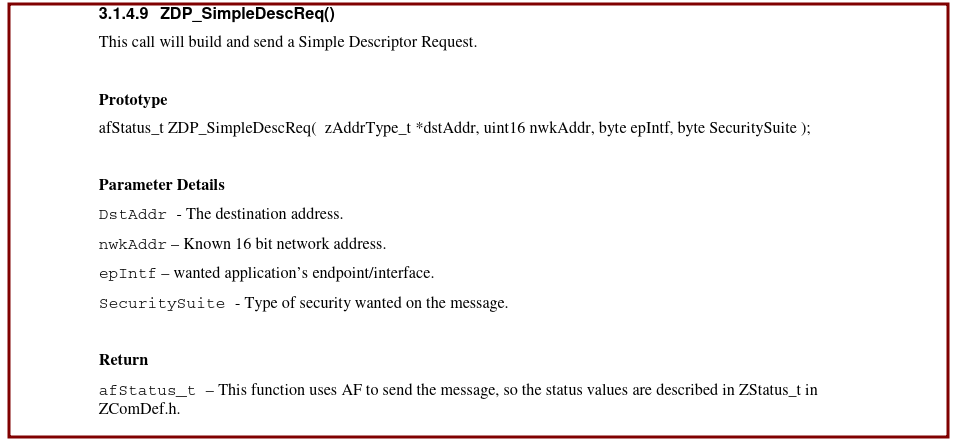
\includegraphics[width=1\textwidth]{media/z-stack-api-excerpt.png}
  \caption{Z-Stack API Auszug}
\end{figure}

In diesem Beispiel wird beschrieben, wie man einen SimpleDescriptor-Request an ein Zigbee-Device versendet. Dieser Aufruf ist entsprechend parametrierbar,
und wird zur Abfrage der verfügbaren Endpunkte eines Gerätes nach dessen Beitritt in das Netzwerk abgefragt.

\subsubsection{zigbee-herdsman}

Der Herdsman ist die eigentliche Kernanwendung von zigbee2mqtt. Diese Modul verbindert sich direkt über einen seriellen Socket mit dem Koordinator. Über diese Schnittstelle
spricht Herdsmann die API des Koordinators an um das Netzwerk zu verwalten. Herdsman verwaltet die Datenbank und damit den Zustand des Netzwerkes. Das Modul stellt nach außen
eine API zur Verfügung, mit der Sich das Netzwerk verwalten lassen kann. Auf diese API greift auch die integrierte WebGui zu.

Die API von Herdman wird im entsprechenden GitHub Repository dokumentiert.
\url{https://github.com/Koenkk/zigbee-herdsman}

\subsubsection{zigbee-herdman-converters}

Dieser Konverter kann proprietäre Cluster die von selbstentwickelten Devices oder manch Devices von Drittherstellern. Mit diesem Converter lassen sich proprietäre Cluster von Geräte
so adaptieren, dass sie nach Wunsch gesteuert und ausgelesen werden können.

\subsubsection{zigbee2mqtt}

Dieses Modul umschreibt die beiden vorher beschriebenen Module und fügt noch eine Weboberfläche hinzu. Die Weboberfläche dient zur Verwaltung und Visualisierung des Netzwerkes.
\begin{figure}[H]
  \centering
  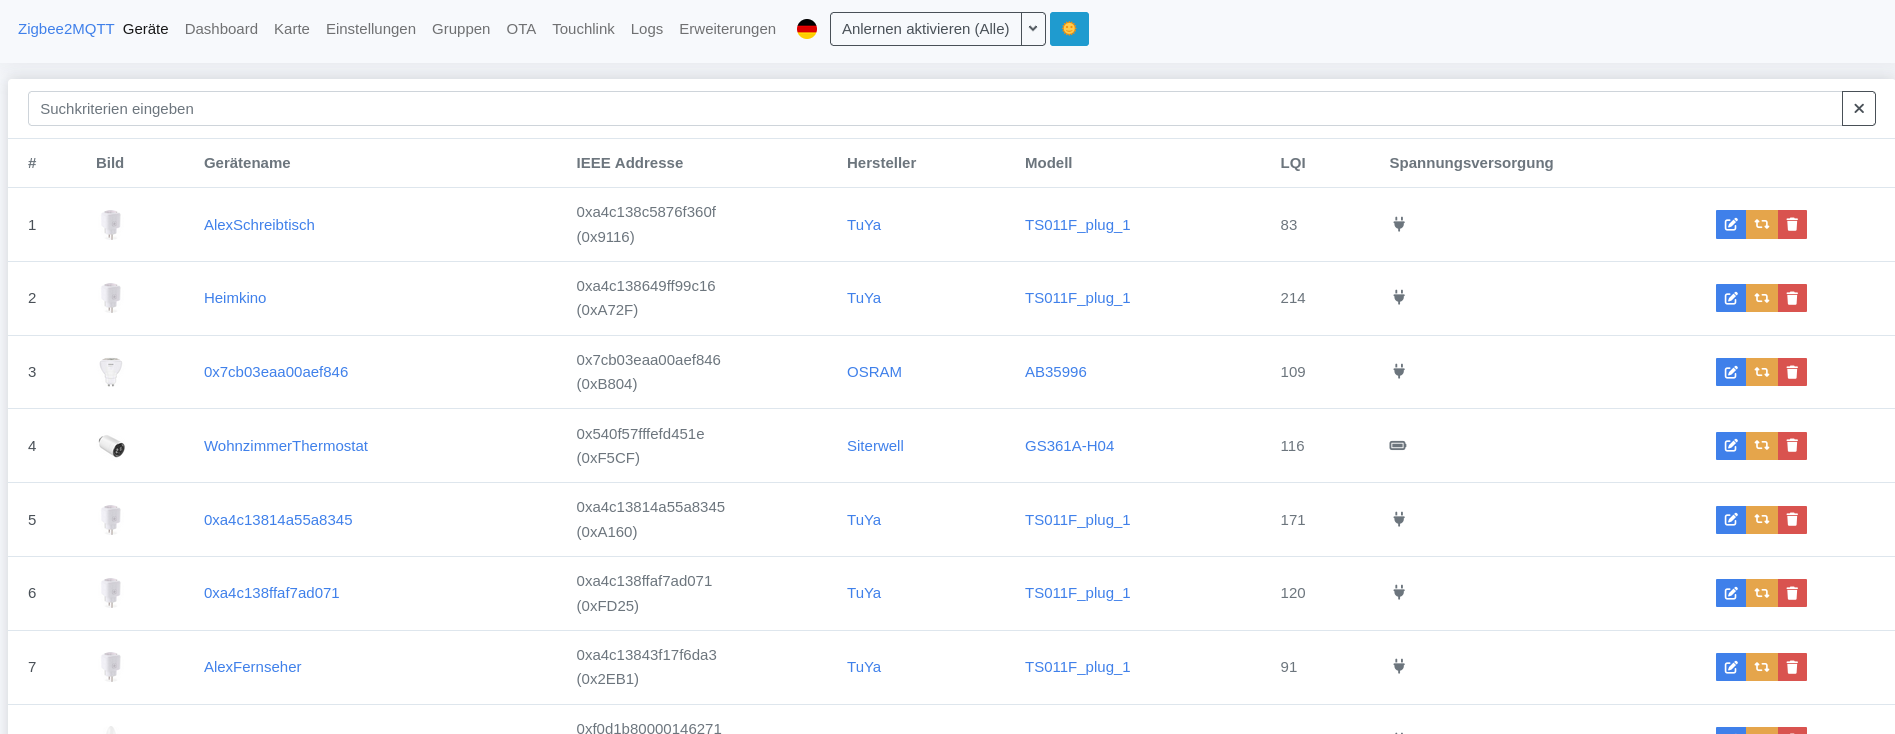
\includegraphics[width=1\textwidth]{media/z2m.png}
  \caption{zigbee2mqtt Webfrontend}
\end{figure}

Die Weboberfläche biete die Möglichkeit alle Endpunkte von Herdsman abzufragen und entsprechend zu steuern.

\begin{figure}[H]
  \centering
  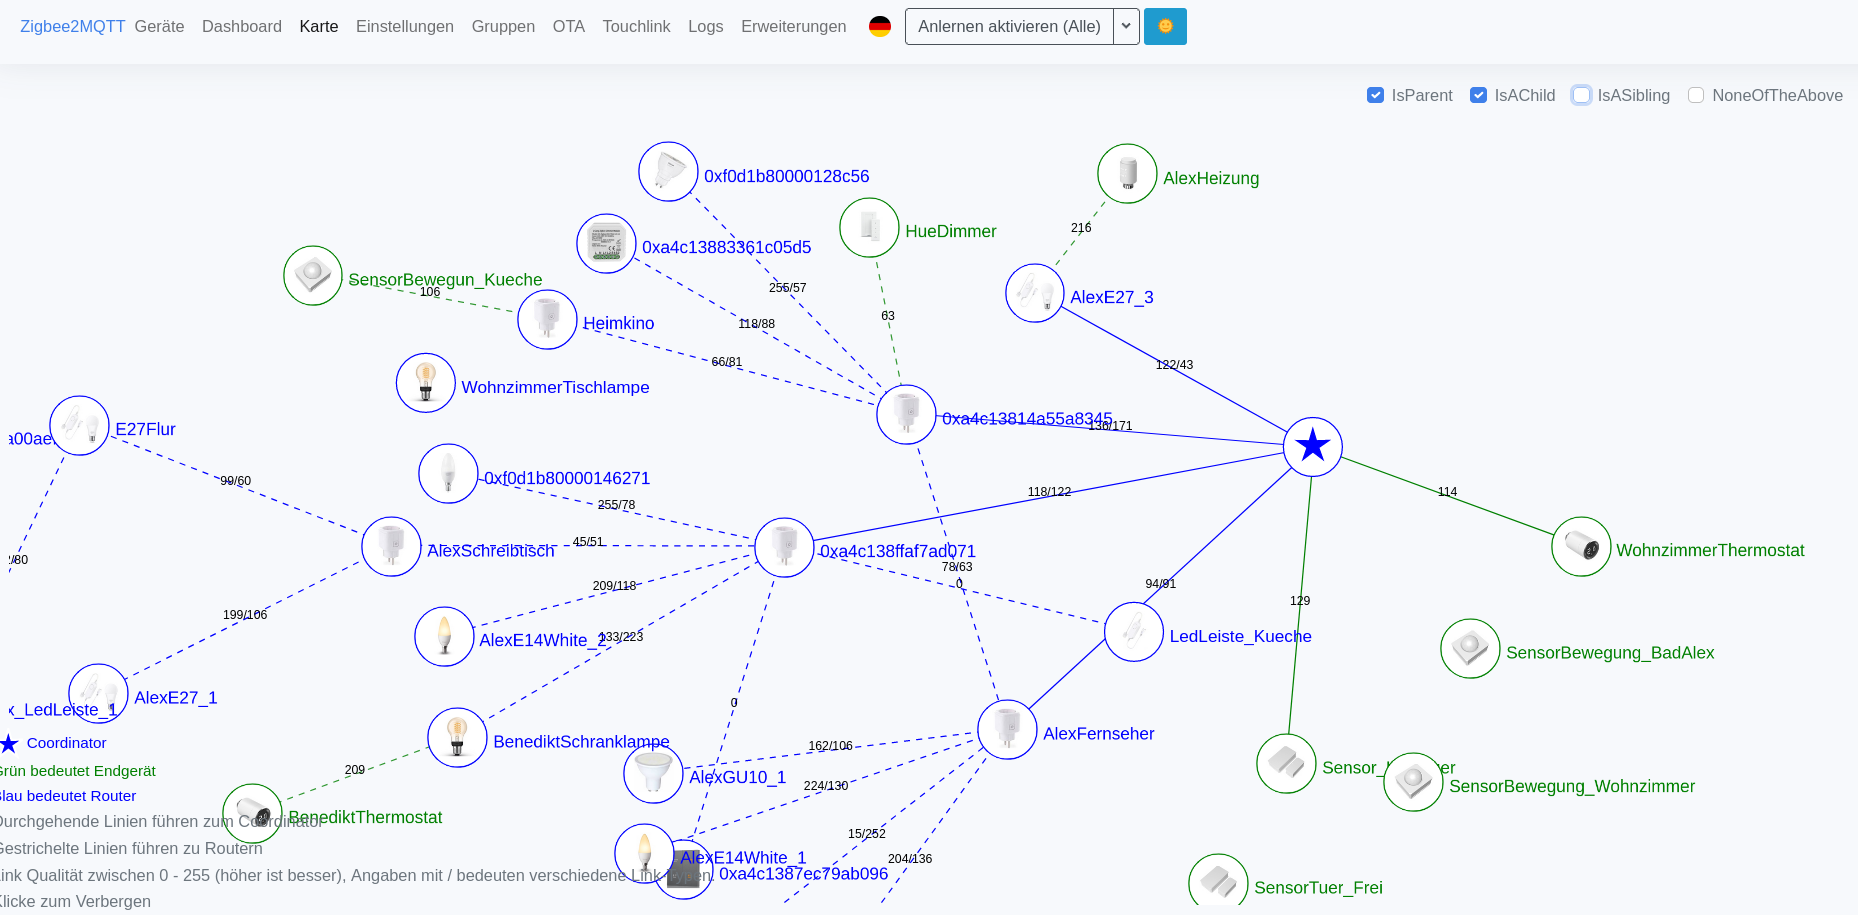
\includegraphics[width=1\textwidth]{media/z2m-map.png}
  \caption{zigbee2mqtt Netzwerkvisualisierung}
\end{figure}

Das Netzwerk lässt sich in einer dynamischen Übersicht visualisieren. Hier die aktiv genutzen Verbindung zwischen den Geräten. 

\subsection{MQTT}

MQTT \cite{mqtt} ist ein Protokoll, um Nachrichten zwischen Teilnehmen in einem Netzwerk auszutauschen. Alle Nachrichten werden unter einem definierten \grqq Topic \grqq{} 
an einen zentralen Messagebroker gesendet. Teilnehmer können \grqq Topics \grqq{} abonnieren. Der Broker verwaltet eine Liste mit allen Teilnehmern sowie 
deren abonnierten \grqq Topics \grqq{}. Wird eine entsprechende Nachricht an den Broker \grqq gepublisht \grqq{}, werden alle \grqq subscriber \grqq{} entsprechend informiert. 

\subsection{Wireshark}

Wireshark ist eine quelloffene Anwendung um Datenstöme Mitzuschneiden und zu Untersuchen. Wireshark selbst nutzt standardmäßig \grqq npcap \grqq{} um Datenverkehr 
auf Netzwerkkarten aufzuzeichnen. Es ist möglich über andere Schnittstellen Wireshark Datenströme zur Verfügung zu stellen. Zu diesem Zweck
können Scripte in den Ordner \grqq .../extcap \grqq{} abgelegt werden, welche 
Paketströme zurückliefern. Diese Technik wird in diesem Versuch eingesetzt.

\begin{figure}[H]
  \centering
  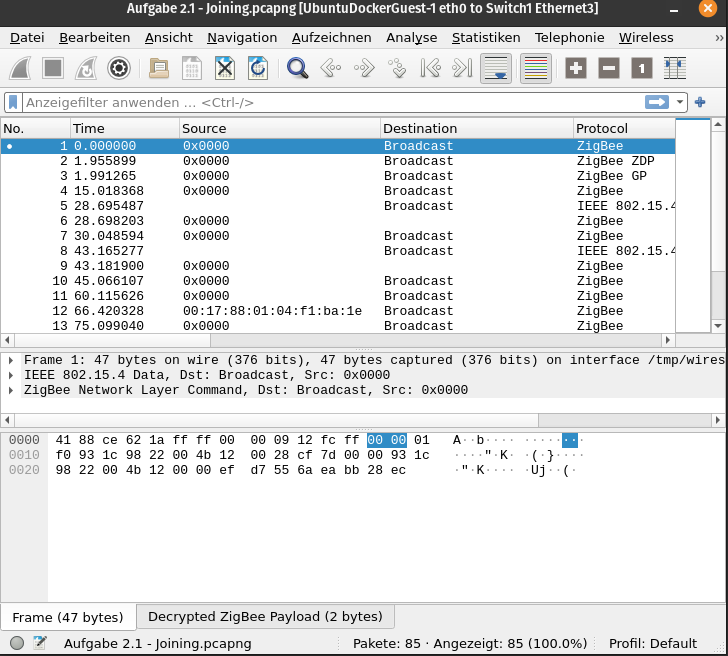
\includegraphics[width=1\textwidth]{media/wireshark.png}
  \caption{Wireshark}
\end{figure}

\subsection{Ansible}

Ansible ist ein Werkzeug zur Automatisierung. Arbeitsabläufe lassen sich strukturiert in YAML (yet another markup language) definieren. Ansible kann Aufgaben auf dem lokalem System und auf Remotesystemen
ausführen. Aufgaben können in Rollen zusammengefasst werden.  
Eine Rolle kann einem Host wie folgt zugewiesen werden:
\begin{lstlisting}
  - name: Deploy the Lab
    hosts: localhost
    roles:
    - DeployDocker
    - DeployLabUtils
\end{lstlisting}

Die Rollen \grqq DeployDocker \grqq{} und \grqq DeployLabUtils \grqq{} umfassen eine Menge von Aufgaben zur Installation notwendiger Komponenten und weitere Vorbereitungen
für den Praktikumsversuch. Diese Rollen werden \grqq localhost \grqq{}, also dem ausführendem System selbst zugewiesen.
Aus technischer Sicht lädt Ansible parametrierte Pythonmodule auf den jewiligen Host per SCP und führt diese dort aus.


